\documentclass{article}   
\usepackage[left=2cm,right=2cm,top=2cm,bottom=2cm]{geometry}



\usepackage[utf8]{inputenc}
\usepackage[spanish,es-noquoting]{babel} %es-noquo... para poner . en equations
\decimalpoint

\usepackage{amssymb}
\usepackage{amsmath}

\usepackage{tabularx}
\usepackage{amsfonts}
\usepackage{array}
\usepackage{graphicx}

\usepackage{multicol}
\usepackage{multirow}

\usepackage{makeidx} % para las tablas de contenidos índices etc


\usepackage{lscape}
\usepackage{float}
\usepackage{array}

\usepackage{lmodern} 
\usepackage{fancyhdr}

\fancypagestyle{plain}{%
	\fancyhf{} % Limpia todos los encabezados y pies de página anteriores
	\renewcommand{\headrulewidth}{0pt} % Sin línea de encabezado
	\renewcommand{\footrulewidth}{0pt} % Sin línea de pie de página
	\fancyfoot[c]{\thepage} % Números de página en la posición central
}



%  usando arial en el trabajo, lo quito para el paper
%\usepackage[T1]{fontenc}
%\usepackage{helvet}

\renewcommand*\familydefault{\sfdefault}
\usepackage{setspace} % interlineados
\usepackage{parskip}  % sangrias 
\setlength{\parindent}{0pt} %sangria párrafos
\onehalfspacing % interlineado total

\usepackage{sectsty}
\sectionfont{\fontsize{12}{15}\selectfont} % Tamaño 12 y espaciado 15
\subsectionfont{\fontsize{12}{15}\selectfont} % Tamaño 12 y espaciado 15

\usepackage{longtable}
\usepackage{booktabs}
\usepackage{ragged2e} 
\usepackage{pdfpages}

%\usepackage{hyperref}

\usepackage[hidelinks]{hyperref} % hidelinks para quitar los bordes de los enlaces


%\usepackage{xcolor}
 \usepackage{listings}
\usepackage{enumitem}
\usepackage{tikz}
\usetikzlibrary{decorations.markings}

\usetikzlibrary{shapes,arrows}
\usetikzlibrary{shapes.geometric, arrows}

\usetikzlibrary{mindmap, trees}
\usetikzlibrary{fadings}
\usetikzlibrary{patterns} %pared compuesta 

\usetikzlibrary{shapes.geometric, arrows.meta, positioning}
\tikzstyle{block} = [rectangle, draw, fill=blue!20, text width=2.5cm, text centered, minimum height=1.5cm, rounded corners]
\tikzstyle{arrow} = [draw, -{Stealth[scale=1.5]}, thick]
\usepackage{pgfplots} %graphs // temperature graph chap5

\usepackage{fontawesome} % Para íconos
%\usepackage{fontawesome5}
%\usetikzlibrary{positioning}



%\usepackage{natbib}

\usepackage{titlesec}

\titleformat{\chapter}[display]
{\normalfont\huge\bfseries}{\chaptertitlename\ \thechapter}{11}{\Huge}
% Establecer el espaciado antes y después de los capítulos
\titlespacing*{\chapter}{0pt}{-40pt}{15pt} % Ajusta el último valor para cambiar el espacio después del título

\usepackage{caption} 


\usepackage{tabularx}
\usepackage{array}
\usepackage{multirow}



\usepackage{etoolbox} % Para modificar la numeración de página
\usepackage{tocbibind}  %numeracion dif


%tabla productos
\usepackage[normalem]{ulem}



 % Configura el punto como separador decimal
\usepackage{siunitx}
\sisetup{output-decimal-marker = {.}}


\usepackage{multirow}
%\usepackage[table,xcdraw]{xcolor}


\usepackage{tocloft}% personalizar indices

% Configurar un índice de ecuaciones con un nombre personalizado (por ejemplo, "eqn")
\newlistof{eqn}{section}{Índice de Ecuaciones}  % Cambiar 'equation' a 'eqn'




\usepackage{graphicx}  
\usepackage{amsmath}  
%%\usepackage{cite}  
\usepackage{abstract} 
\usepackage{multicol}

\usepackage{ragged2e}

\title{Diseño y Selección de Materiales para una Cámara de Refrigeración para la Conservación de Insulina en la UMF 40, Azcapotzalco, CDMX}  
\author{Monjaraz Ramírez Israel}  
\date{02 de diciembre de 2024}  




\usepackage{tikz}
\usetikzlibrary{arrows.meta, shapes.geometric, positioning, calc}

% Configuración básica de estilos
\tikzset{
	axis/.style={thick, ->},               % Estilo para ejes
	cycle/.style={thick, blue},            % Estilo para líneas de ciclos
	isentrope/.style={dashed, gray},       % Estilo para líneas isentrópicas
	point/.style={circle, fill=red, inner sep=1.5pt}, % Puntos clave
	label/.style={font=\small}             % Estilo para etiquetas
}

\usepackage{lmodern} 
\usepackage{apacite}
\begin{document}

\maketitle

\justifying

\section*{Resumen}
Este trabajo presenta el diseño y desarrollo de una cámara de refrigeración médica destinada a la conservación de insulina en la UMF40 Santa Bárbara, Azcapotzalco, CDMX. La selección adecuada de materiales para la construcción del equipo es crucial para garantizar un almacenamiento seguro y eficiente de la insulina. Se detallan los criterios para la elección de materiales que optimicen la eficiencia energética, el aislamiento térmico y la durabilidad del sistema. Además, se discuten las aplicaciones prácticas de estos materiales dentro del contexto médico, asegurando que la cámara mantenga condiciones de temperatura estables y dentro de los rangos adecuados para preservar la efectividad de la insulina.

\section*{Abstract}
This paper presents the design and development of a medical refrigeration chamber for the storage of insulin at UMF40 Santa Bárbara, Azcapotzalco, CDMX. The appropriate selection of materials for the construction of the equipment is crucial to ensure safe and efficient insulin storage. The criteria for choosing materials that optimize energy efficiency, thermal insulation, and system durability are detailed. Furthermore, the practical applications of these materials within the medical context are discussed, ensuring that the chamber maintains stable temperature conditions within the appropriate range to preserve the effectiveness of the insulin.

\begin{multicols}{2}
	
	\section{Introducción}
La refrigeración es un proceso fundamental para la conservación de alimentos, medicamentos y otros productos sensibles a la temperatura. Este proceso consiste en la transferencia de calor desde un espacio confinado hacia un entorno de mayor temperatura, permitiendo mantener condiciones controladas dentro del sistem\cite{caloryfrio-2018}. \\

En el ámbito médico, la refrigeración desempeña un papel crucial en la conservación de medicamentos como la insulina, una hormona esencial para el tratamiento de la diabetes mellitus. La insulina debe mantenerse entre $2^\circ$C y $8^\circ$C para preservar su efectividad; temperaturas fuera de este rango pueden provocar la desnaturalización de la proteína, inutilizando el medicamento.\\
La Ciudad de México presenta retos particulares debido a su altitud (2250 m sobre el nivel del mar) y temperaturas promedio entre $12^\circ$C y $27^\circ$C. Estas condiciones afectan el diseño de los sistemas de refrigeración, ya que la presión atmosférica más baja disminuye la eficiencia de los compresores y condensadores. Esto resalta la necesidad de sistemas que no solo sean eficientes, sino también adaptados a las condiciones locales.\\
Un diseño eficiente de sistemas de refrigeración para equipos médicos requiere una cuidadosa selección de materiales y el uso de simulaciones térmicas avanzadas. En particular, la ciencia de materiales desempeña un papel clave en el desarrollo de componentes como aislantes térmicos, recubrimientos internos y externos, y sellos herméticos. Materiales como el poliuretano expandido, con su baja conductividad térmica y alta resistencia al envejecimiento, son ideales para reducir las pérdidas térmicas. Asimismo, el uso de recubrimientos de acero inoxidable garantiza la durabilidad estructural y la resistencia a la corrosión, indispensables en entornos médicos.\cite{dincer-2016}\\

La validación de estos sistemas se realiza mediante simulaciones térmicas detalladas que evalúan el flujo de calor, las distribuciones de temperatura y el comportamiento del sistema bajo diferentes escenarios de operación. Herramientas como ANSYS permiten optimizar el diseño antes de la construcción, minimizando riesgos y garantizando el cumplimiento de normativas internacionales en equipos médicos. Estas simulaciones también identifican posibles fallas, mejorando la confiabilidad y prolongando la vida útil del equipo.\cite{Dincer2010-re} \\

En este contexto, la integración de principios de ciencia de materiales y simulación térmica permite desarrollar cámaras de refrigeración más eficientes y seguras, asegurando la conservación de medicamentos críticos como la insulina en condiciones óptimas, incluso en escenarios desafiantes como los presentados por la Ciudad de México. \cite{ashrae-about}


\begin{figure}[H]
	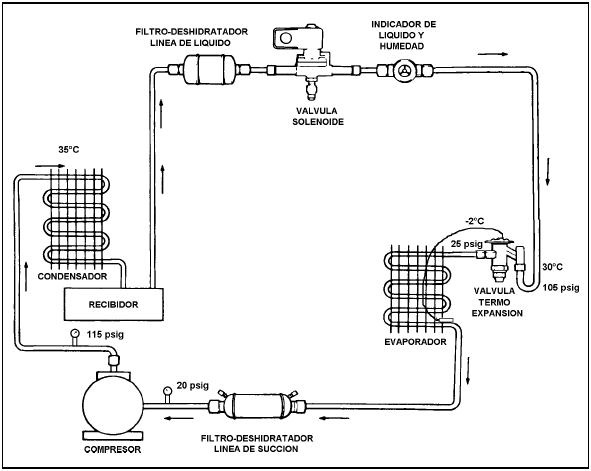
\includegraphics[width=\linewidth]{figures/ciclo-ref.png}
	\caption{Ciclo de refrigeración}
	\label{fig:ciclo}	
\end{figure}

	\begin{figure}[H]
	\centering
	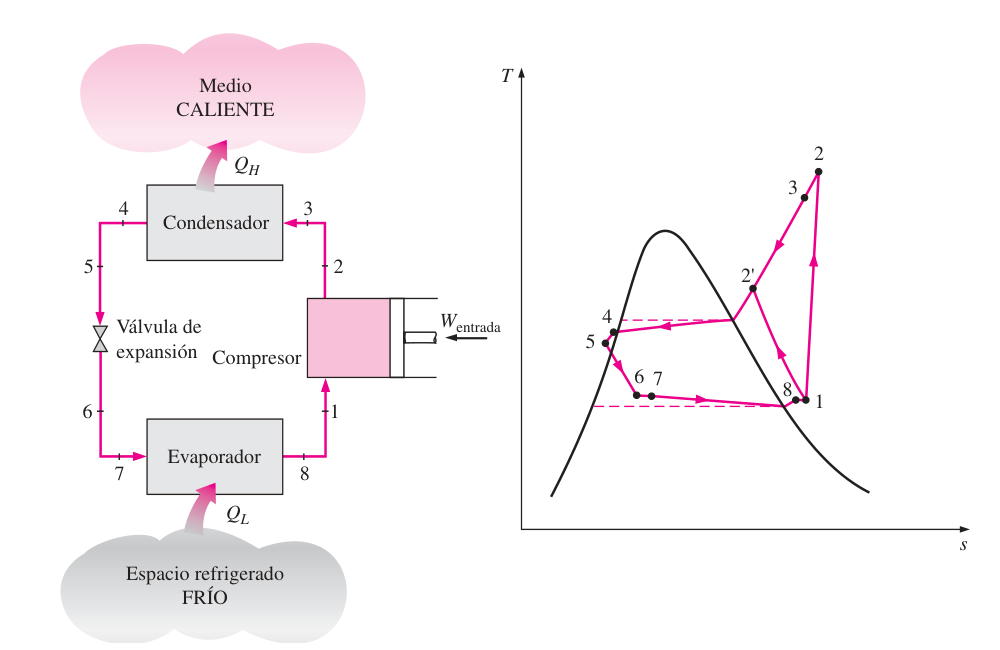
\includegraphics[width=\linewidth]{figures/diag-ts}
	\caption{Diagrama T-S del ciclo de refrigeración}
	\label{fig:diag-ts}x
\end{figure}


	\section{Diseño Experimental de la Cámara de Refrigeración}
	La cámara propuesta tiene dimensiones de 50x60x60 cm y está diseñada para manejar una carga térmica total de 3500 BTU. El diseño se divide en tres aspectos principales: aislamiento térmico, sistema de refrigeración y pruebas experimentales.


	
	\begin{figure}[H]
		\centering
		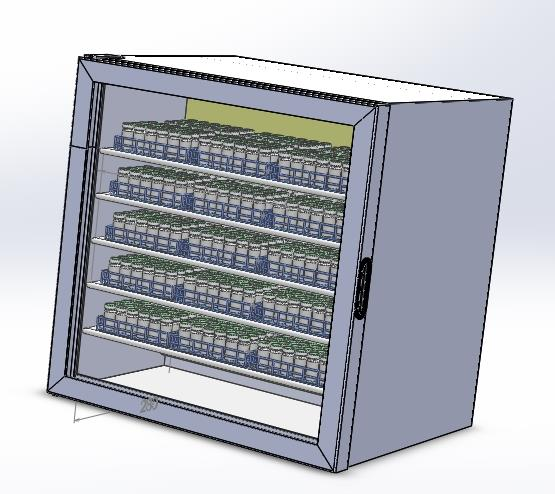
\includegraphics[width=\linewidth]{figures/axo-parrilasycharolas}
		\caption{Vista general de la cámara de refrigeración}
		\label{fig:vista-camara}
	\end{figure}
	
	
	
	\subsection{Cálculo de la Carga Térmica}
	El cálculo de la carga térmica considera:
	\[
	Q = U \cdot A \cdot (T_{\text{int}} - T_{\text{ext}}) + Q_{\text{ocupantes}} + Q_{\text{equipos}} 
	\]
	donde:
	\begin{itemize}
		\item $Q$: carga térmica total (BTU).
		\item $U$: coeficiente de transmisión térmica del material (BTU/h-ft$^2$-$^\circ$F).
		\item $A$: área total del aislamiento (ft$^2$).
		\item $T_{\text{int}}$ y $T_{\text{ext}}$: temperaturas interior y exterior ($^\circ$F).
		\item $Q_{\text{ocupantes}}$: carga generada por ocupantes (negligible en este caso).
		\item $Q_{\text{equipos}}$: carga generada por equipos internos (negligible).
	\end{itemize}
	
	Para materiales con $U$ bajo (como el poliuretano expandido), se reduce significativamente la transferencia de calor.
	
 	
	
\begin{table}[H]
	\centering
	\caption{Comparación de Materiales de Aislamiento Térmico}
 
\setlength{\tabcolsep}{5pt} % Ajusta el espacio entre columnas (puedes aumentar o disminuir)
\begin{tabular}{|l|l|}
	\hline
	\textbf{Material} & \textbf{Propiedades} \\ \hline
	\textbf{Poliuretano Expandido} & Conductividad térmica: 0.02 W/mK \\ \hline
	\textbf{Acero Inoxidable} & Alta resistencia a la corrosión. \\ \hline
	\textbf{Juntas de Silicona} & Material flexible, alta capacidad de sellado \\ \hline
\end{tabular}
	
	\vspace{0.11cm} % Espacio entre la tabla y la sección de Ventajas
	
	\begin{tabular}{|l|}
		\hline
		\textbf{Ventajas} \\ \hline
		Excelente aislamiento con espesores pequeños \\ \hline
		Durabilidad y resistencia a ambientes agresivos \\ \hline
		Garantiza hermeticidad y previene pérdidas térmicas \\ \hline
	\end{tabular}
\end{table}




	\subsection{Selección de Materiales}
	\begin{itemize}
		\item \textbf{Aislamiento térmico:} Poliuretano expandido con una conductividad térmica de 0.02 W/mK, que ofrece un excelente aislamiento con espesores pequeños.
		\item \textbf{Recubrimientos internos y externos:} Acero inoxidable, elegido por su resistencia a la corrosión y facilidad de limpieza.
		\item \textbf{Sellado:} Uso de juntas de silicona para garantizar hermeticidad y prevenir pérdidas térmicas.
	\end{itemize}
	
 \begin{figure}[H]
 	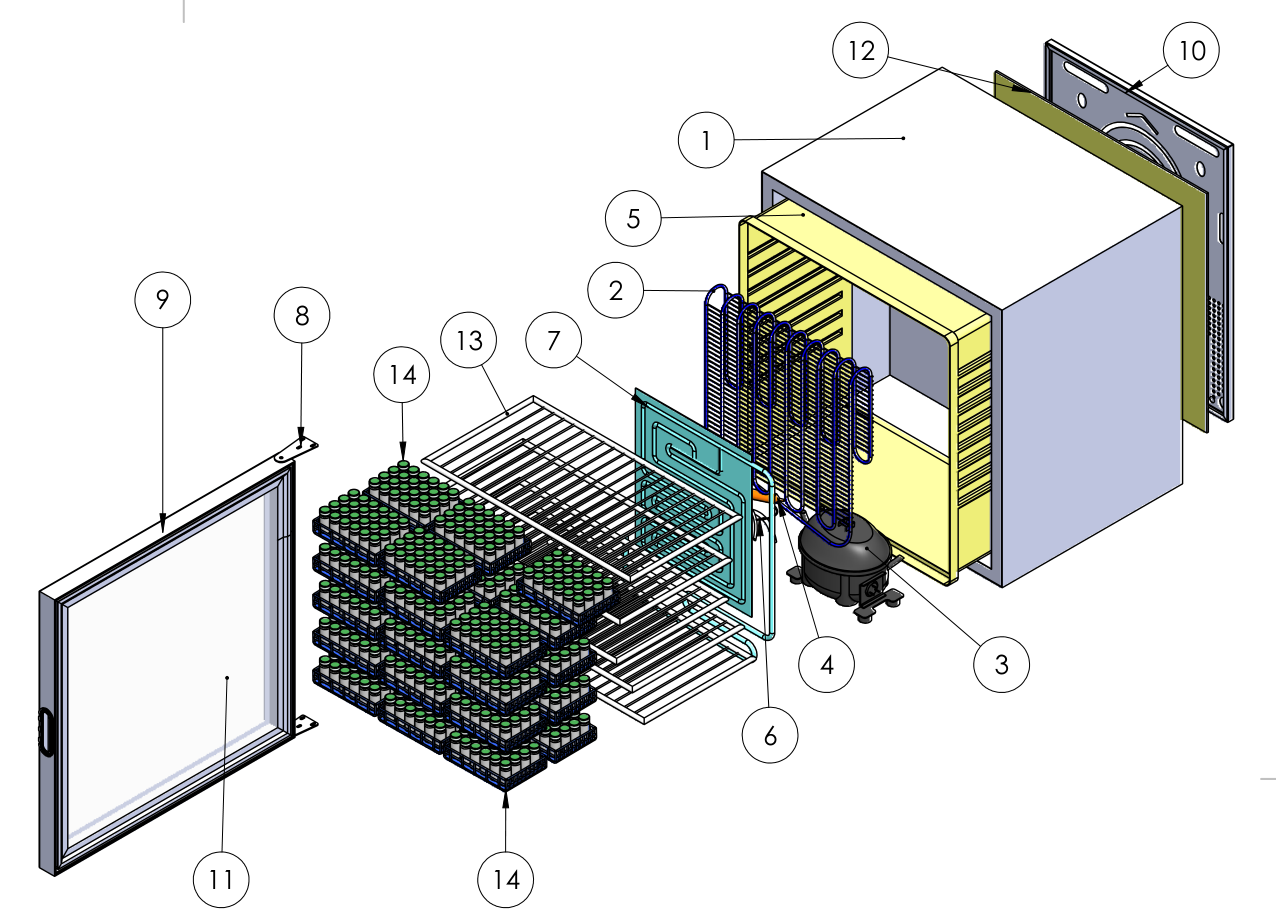
\includegraphics[width=\linewidth]{figures/front-chapetr4.png}
 	\caption{Equipo de refrigeración diseñado}
 \end{figure}
 
	\subsection{Simulación y Evaluación de Materiales}
	Para validar el diseño, se realizaron simulaciones térmicas usando software como ANSYS, evaluando la distribución de temperatura y el flujo de calor. Además, se realizaron pruebas de impacto para garantizar que el recubrimiento resista deformaciones. \cite{areatecnologia}
	

 \begin{figure}[H]
 	\centering
 	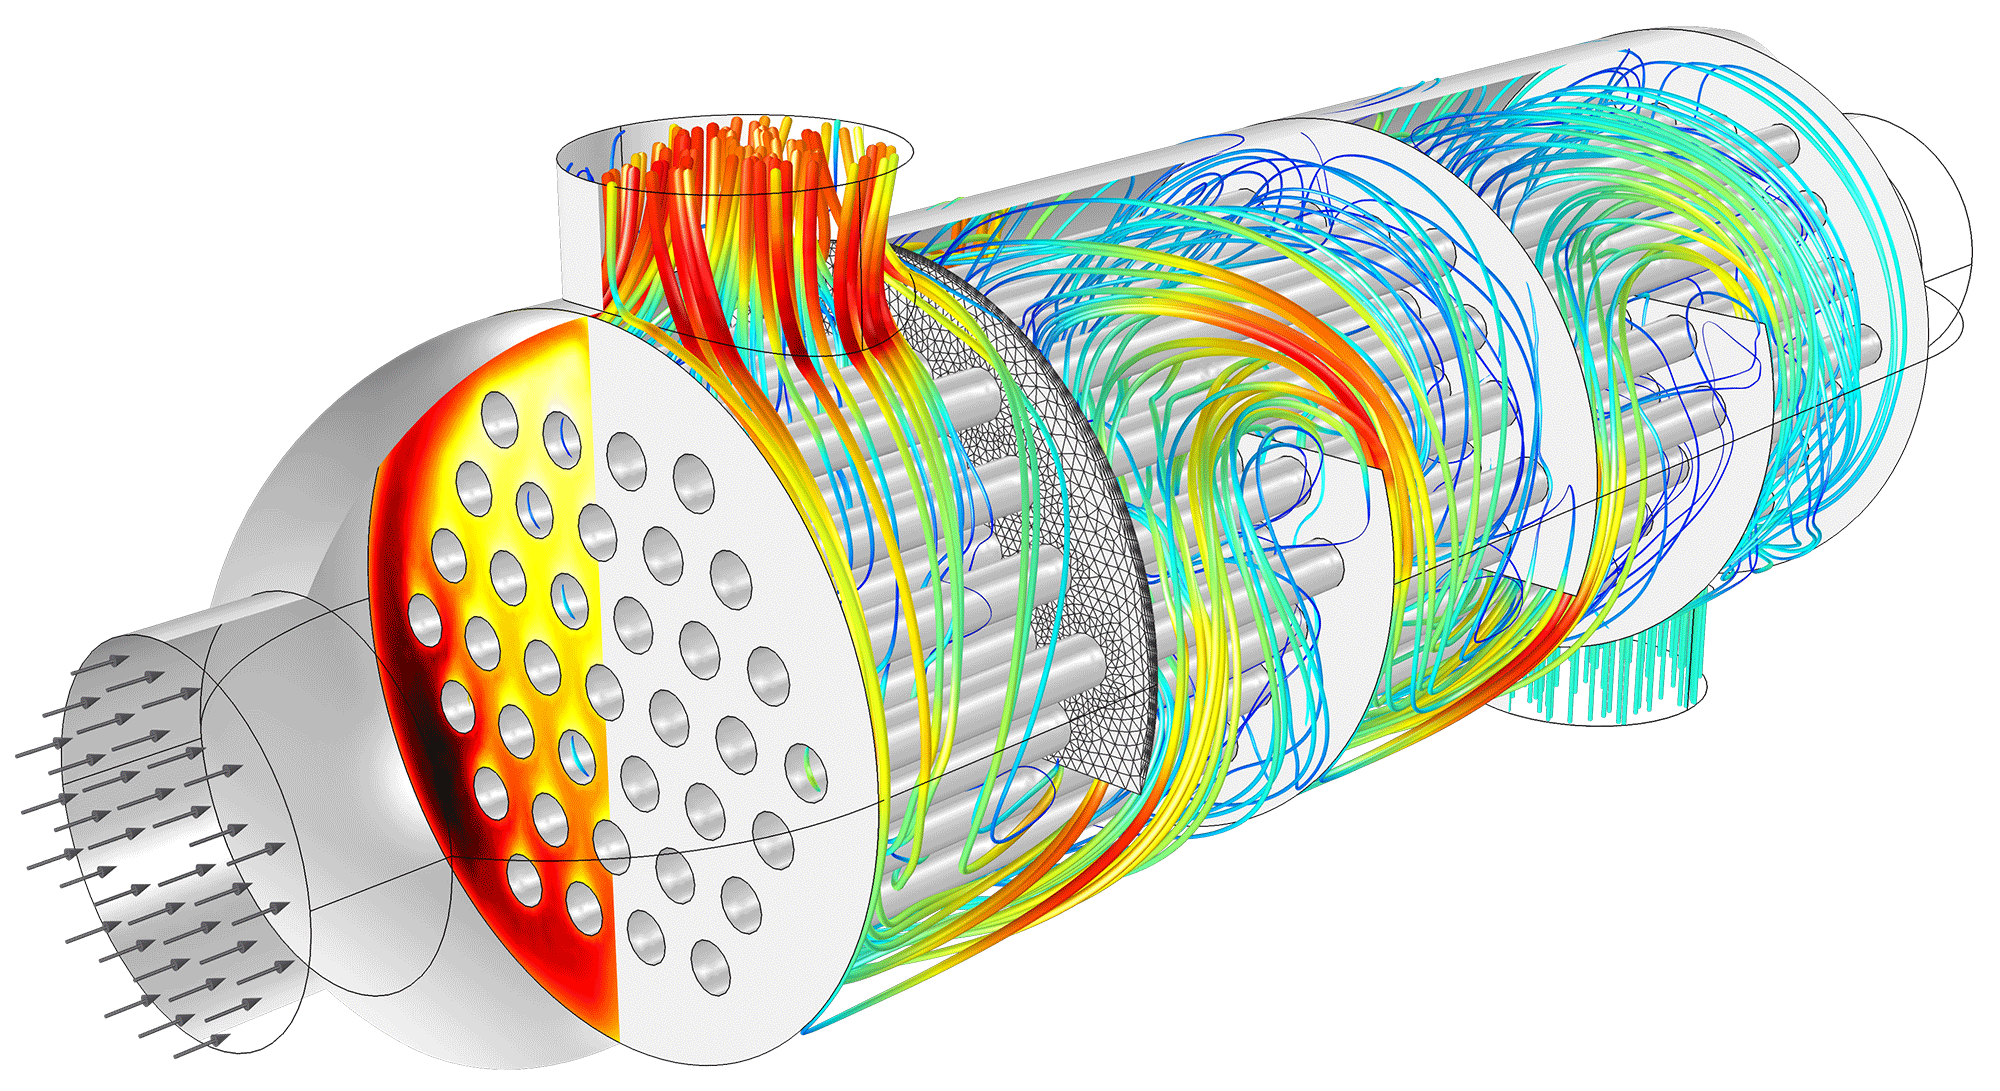
\includegraphics[width=\linewidth]{figures/dist-intcalor}
 	\caption{Simulación de intercambiador de calor.}
 	\label{fig:dist-intcalor}
 \end{figure}
 
 	\begin{figure}[H]
		\centering
		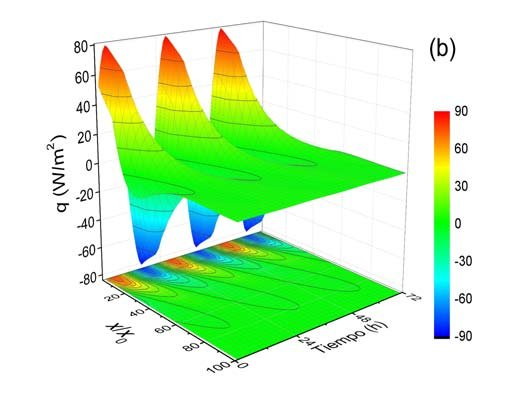
\includegraphics[width=\linewidth]{figures/temp-simulation}
		\caption{Distribución espacio-temporal del flujo de calor por unidad de área, en función del tiempo.}
		\label{fig:temp-simulation}
	\end{figure}
	
	
	\section{Resultados y Discusión}
	\subsection{Eficiencia Energética}
	El sistema diseñado mantiene una temperatura estable de $4^\circ$C con un consumo energético optimizado. Las simulaciones muestran que el poliuretano reduce las pérdidas térmicas en un 30\% en comparación con materiales tradicionales.
	
	\subsection{Impacto de la Altitud}
	La altitud disminuye la presión del aire, lo que afecta la capacidad del condensador y el compresor. Sin embargo, el condensador Modelo: CH111*B - CH501*B de temperatura Baja,  compensó adecuadamente estas pérdidas. \cite{bohn}
	
\subsection{Pruebas de Resistencia}
Las pruebas de resistencia realizadas garantizaron la durabilidad y funcionalidad de la cámara bajo diferentes condiciones de operación, evaluando tanto los recubrimientos externos como el aislamiento térmico. Estas pruebas se diseñaron para simular escenarios reales e intensivos que podrían presentarse durante la vida útil del equipo.

\subsubsection*{Pruebas de impacto mecánico}
Se realizaron simulaciones para evaluar la resistencia de los recubrimientos externos de acero inoxidable frente a impactos accidentales y vibraciones típicas en entornos médicos. Usando análisis de elementos finitos (FEM) en ANSYS, se aplicaron cargas puntuales y distribuidas que representaban golpes comunes, como el contacto con equipos rodantes o caídas de objetos.

Los resultados mostraron que el recubrimiento puede soportar fuerzas de hasta 50 N sin sufrir deformaciones permanentes, manteniendo su integridad estructural. Esto asegura que la cámara pueda operar de forma segura en ambientes exigentes.

\subsubsection*{Pruebas de presión interna}
Para garantizar la hermeticidad del sistema, se sometió a la cámara a variaciones de presión interna que simulan el cierre brusco de la puerta. Estas pruebas confirmaron que los sellos de silicona evitan fugas de aire incluso después de 10,000 ciclos de apertura y cierre, manteniendo la estabilidad térmica en su interior.

\subsubsection*{Pruebas de ciclos térmicos}
El aislamiento térmico de poliuretano expandido fue evaluado mediante ciclos de calentamiento y enfriamiento entre $-5^\circ$C y $40^\circ$C, reproduciendo escenarios extremos de operación. Estas pruebas permitieron identificar posibles deformaciones, agrietamientos o pérdidas de propiedades aislantes del material.

El análisis demostró que el aislamiento conserva su rendimiento térmico después de más de 500 ciclos, sin evidencias de degradación significativa. Esto valida la durabilidad del material incluso bajo condiciones fluctuantes.

\subsubsection*{Pruebas de envejecimiento acelerado}
Se realizaron pruebas de envejecimiento acelerado exponiendo los materiales a humedad relativa del 90\% y temperaturas constantes de $30^\circ$C durante un periodo simulado de 5 años. Los resultados indicaron que tanto los recubrimientos como los sellos de silicona y el aislamiento térmico mantienen más del 95\% de sus propiedades originales después del periodo de simulación, asegurando su funcionalidad a largo plazo.

\subsubsection*{Pruebas de carga estructural}
Se evaluó la capacidad de la cámara para soportar cargas estáticas y dinámicas, como el peso de equipos médicos colocados sobre su superficie. Los análisis confirmaron que la estructura puede soportar hasta 30 kg sin deformaciones significativas, proporcionando una base sólida para su integración en hospitales o clínicas.

	
	\section{Conclusión}
	El diseño y selección de materiales garantizan un sistema eficiente, confiable y adaptado a las condiciones ambientales de la Ciudad de México. Este enfoque asegura que la insulina se conserve en óptimas condiciones, mejorando la seguridad y la vida útil del medicamento. El uso de ANSYS en el diseño y validación de la cámara no solo garantizó un desempeño térmico eficiente, sino también una estructura confiable y duradera, cumpliendo con los estándares médicos más exigentes.
	
	
	\section*{Referencias}
	
\bibliographystyle{apacite}  % Estilo APA
\bibliography{referencias}
\begin{enumerate}[label=\arabic*.]
\setlength\itemsep{1em} % Espacio entre elementos
\item \begin{flushleft} \textbf{Curiosfera.} (2023). Historia de la refrigeración. \textit{https://curiosfera-historia.com/historia-de-la-refrigeracion/}. \end{flushleft}
\item \begin{flushleft} \textbf{DataMéxico.} (2022). Insulina y sus Sales: Intercambio comercial, compras y ventas internacionales, mercado y especialización | Data México. Descargado de \textit{https://www.economia.gob.mx/datamexico/es/profile/product/their-insulin-and-sales}. \end{flushleft}
\item \begin{flushleft} \textbf{Instituto Nacional de Estadística y Geografía, I. N.} (2024, 26 de enero). Estadísticas de defunciones registradas (edr). \textit{https://www.inegi.org.mx/contenidos/saladeprensa/boletines/2024/EDR/EDR2023_En-Jn.pdf. ([Nota de prensa])}. \end{flushleft}
\item \begin{flushleft} \textbf{De Leon, E.} (2017). Construcción y diseño de una cámara frigorífica. Descargado de \textit{https://www.edificacionescien.com/es/blog-cien-3/33-construccion-y-diseno-de-una-camara-frigorifica.html}. \end{flushleft}
\item \begin{flushleft} \textbf{Secretaría de Salud, S.} (2022, 8). Normas oficiales mexicanas. \textit{https://www.gob.mx/salud/en/documentos/normas-oficiales-mexicanas-9705}. \end{flushleft}
\item \begin{flushleft} \textbf{Diario Oficial de la Federación (DOF).} (2010, noviembre 23). NOM-008-SCFI-2002: Sistema general de unidades de medida. (Ciudad de México). \end{flushleft}
\item \begin{flushleft} \textbf{Diario Oficial de la Federación DOF.} (2010, noviembre 23). NOM-012-ENER-2019: Eficiencia energética de unidades condensadoras y evaporadoras para refrigeración. Límites, métodos de prueba y etiquetado. (Ciudad de México). \end{flushleft}
\item \begin{flushleft} \textbf{Diario Oficial de la Federación (DOF).} (2010, noviembre 23). NOM-015-SSA2-2010: Para la prevención, tratamiento y control de la diabetes mellitus. (Ciudad de México). \end{flushleft}
\item \begin{flushleft} \textbf{Dincer, I., y Kanoglu, M.} (2010). \textit{Refrigeration systems and applications 2e: Dinçer/refrigeration systems and applications}. Hoboken, NJ, Estados Unidos de América: Wiley-Blackwell. \end{flushleft}
\item \begin{flushleft} \textbf{Dinçer, I., y Kanoglu, M.} (2010). \textit{Refrigeration systems and applications}. United Kingdom: John Wiley and Sons Inc. \end{flushleft}
\item \begin{flushleft} \textbf{DOI.} (1952). Report of the commissioner of patents for the year 1951. \end{flushleft}
\item \begin{flushleft} \textbf{Ecoproyecta.} (2024, 8 de enero). Plan director de los pozos de la ni. \end{flushleft}
\end{enumerate}

\end{multicols}

\end{document}
